\documentclass[conference]{IEEEtran}

\usepackage{xspace}
\usepackage{ifpdf}
\usepackage{diagbox}
\usepackage{cite}
\ifCLASSINFOpdf
  \usepackage[pdftex]{graphicx}
  \DeclareGraphicsExtensions{.pdf,.jpeg,.png}
\else
  \usepackage[dvips]{graphicx}
  \DeclareGraphicsExtensions{.eps}
\fi 
\usepackage[cmex10]{amsmath}
\usepackage{algorithmic}
\usepackage{array}
\usepackage{mdwmath}
\usepackage{mdwtab}
\usepackage{eqparbox}
\usepackage{fixltx2e}
\usepackage{hyperref}
\usepackage{booktabs}
\usepackage{numprint}
\npdecimalsign{.} 
\npthousandsep{,} 
% \usepackage{stfloats} 
\usepackage{xspace}

\newcommand{\Rascal}{\textsc{Rascal}}
% \newcommand{\DCFlow}{\textsc{DCFlow}\xspace}
\newcommand{\DeFacto}{\textsc{DeFacto}\xspace}
      
% *** SUBFIGURE PACKAGES ***
%\usepackage[tight,footnotesize]{subfigure}
% subfigure.sty was written by Steven Douglas Cochran. This package makes it
% easy to put subfigures in your figures. e.g., "Figure 1a and 1b". For IEEE
% work, it is a good idea to load it with the tight package option to reduce
% the amount of white space around the subfigures. subfigure.sty is already
% installed on most LaTeX systems. The latest version and documentation can
% be obtained at:
% http://www.ctan.org/tex-archive/obsolete/macros/latex/contrib/subfigure/
% subfigure.sty has been superceeded by subfig.sty.
  
%\usepackage[caption=false]{caption}
%\usepackage[font=footnotesize]{subfig}
% subfig.sty, also written by Steven Douglas Cochran, is the modern
% replacement for subfigure.sty. However, subfig.sty requires and
% automatically loads Axel Sommerfeldt's caption.sty which will override
% IEEEtran.cls handling of captions and this will result in nonIEEE style
% figure/table captions. To prevent this problem, be sure and preload
% caption.sty with its "caption=false" package option. This is will preserve
% IEEEtran.cls handing of captions. Version 1.3 (2005/06/28) and later 
% (recommended due to many improvements over 1.2) of subfig.sty supports
% the caption=false option directly:
\usepackage[caption=false,font=footnotesize]{subfig}
%
% The latest version and documentation can be obtained at:
% http://www.ctan.org/tex-archive/macros/latex/contrib/subfig/
% The latest version and documentation of caption.sty can be obtained at:
% http://www.ctan.org/tex-archive/macros/latex/contrib/caption/

\hyphenation{op-tical net-works semi-conduc-tor}
\usepackage{etex}  
\usepackage{amssymb}
\usepackage{multicol}
\usepackage{mathrsfs}
\usepackage{microtype}
\usepackage{tabularx}
\usepackage{comment}
\usepackage{synttree}
\usepackage{stmaryrd}
\usepackage{wrapfig}

%% REMOVE PAGE NUMBERS!
\pagestyle{plain}

\newcommand{\loc}[1]{\small{\texttt{#1}}\xspace}
\newcommand{\mthree}{\ensuremath{M^3}\xspace}

\begin{document}

\title{{\huge $M^3$: A General Model for Source Code Analytics in Rascal}}

% author names and affiliations
% use a multiple column layout for up to three different
% affiliations
% TODO: Other authors?
%\author{ Anastasia Izmaylova, Paul Klint, Ashim Shahi and Jurgen Vinju, Davy, Michael}
\author{
\IEEEauthorblockN{Mark Hills\IEEEauthorrefmark{1}}
\IEEEauthorblockA{\IEEEauthorrefmark{1}East Carolina University, Greenville, NC, USA\\mhills@cs.ecu.edu}
\and
\IEEEauthorblockN{Paul Klint, Davy Landman, Michael Steindorfer}
\IEEEauthorblockN{Ashim Shahi, Jurgen Vinju\IEEEauthorrefmark{2}}
\IEEEauthorblockA{\IEEEauthorrefmark{2}Centrum Wiskunde \& Informatica, Amsterdam, The Netherlands\\\{Paul.Klint,Davy.Landman,Michael.Steindorfer,\\Ashim.Shahi,Jurgen.Vinju\}@cwi.nl}
}

\maketitle

\section{Motivation}

In the context of the EU FP7 project ``OSSMETER'' we have developed an infra-
structure for measuring source code. The goal of OSSMETER is to obtain insight
in the quality of open-source projects from all possible perspectives, including product, process and community\footnote{\url{http://www.ossmeter.org}}. 

The three challenges that our part of the design, which focuses on source code, faced
are \emph{variability}, \emph{integration} and \emph{accuracy} \textbf{NOTE: we have accuracy in here to distance ourselves from the srcML approach, variability is a given and integration is here due to the Call for Papers}:
\begin{itemize}
\item[Variability] is necessary to support the different languages and their dialects we support, as well as the different metrics we will compute.
\item[Integration] is necessary at a semantic level, where metrics are computed across programming language and domain boundaries, and are combined for further analysis.
\item[Accuracy] is a prerequisite for insightful analyses. When accuracy is lost in the early stage of fact extraction from source code, the downstream analyses may show interesting but nevertheless meaningless information.
\end{itemize}
%
The standard solution for variability and integration is to put an explicit reusable model
(database, graph) in between such that model producers (parsers \& extractors)
can be de-coupled from model consumers (metrics \& visuals). Examples of such intermediate models are FAMIX~\cite{famix}, RSF~\cite{rsf}, GXL~\cite{GXL}, and KDM~\cite{KDM}, ATerms~\cite{aterms} and
S-Expressions~\cite{sexpr}. A positive side-effect of intermediate models is that the data is pushed into a general form, this also enables integrating information from different sources. We have been inspired by these examples.

This abstract is a brief description of \mthree, a set of code models, which should be easy to
construct, easy to extend to include language specifics and easy to consume to produce metrics and other analyses\footnote{An earlier shorter version of the current abstract on \mthree has been presented earlier at BENEVOL 2014 (no formal proceedings).}. \mthree consists of a abstract syntax tree (AST) layer (hierarchical) and a relational (flat) layer. The AST layer is standardized on interface, but expected to be language specific, while the relational layer is more abstract in nature and made for reuse.

\emph{The main threat to validity of any intermediate model which is generic enough to be reusable between different programming languages is that accuracy may be lost. This is why the \mthree standard first prescribes precise language-specific AST models and then language agnostic relational models where it is possible to abstract.}
The reader should be aware that we do \emph{not} intend to
create a unified model for programming language semantics. Such a language
independent model would be inaccurate (wrong), and deliver meaningless
metrics. Instead we opt for a unified \emph{form} for storing facts about
programs. This means that all models will have a predictable shape, but we do
not assume any reusability of metrics or visuals producers between models
produced by different parsers. The design of \mthree  gives accuracy a higher priority than reuse.

\begin{figure}[t]
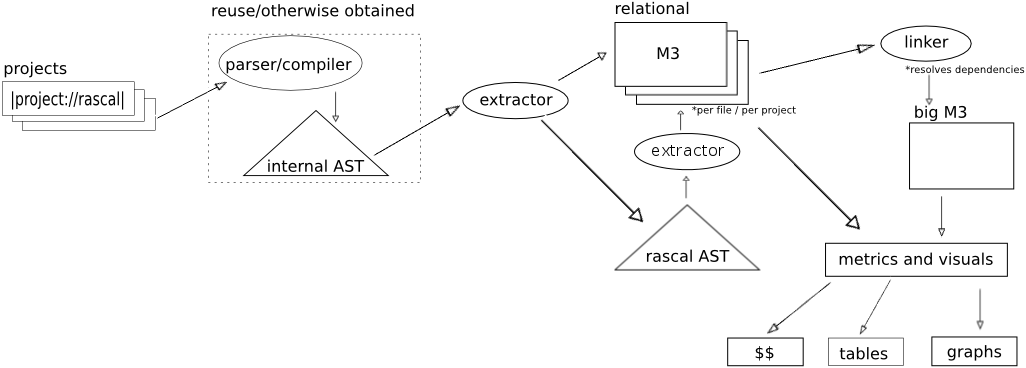
\includegraphics[width=\columnwidth]{m3}
\caption{An overview: from code to metrics and visuals via M3 models.}
\end{figure}

The context of \mthree\ is the Rascal meta-programming 
language~\cite{KvdSV- Rascal11,rascalscam}.\footnote{\url{http://www.rascal-mpl.org}} 
This is a
domain specific language specifically designed to include primitives we need
to model any programming language syntax and semantics, and to analyze and
manipulate these models. Three essential design elements for the purpose of
this paper are that Rascal has value semantics for all in-memory data,
including sets and relations, it has support for URI literals, called ``source
locations'', and it has term rewriting and relational calculus primitives to
deal with hierarchical and relational data, respectively. This includes
generic traversal~\cite{scrap,travfuncs} and pattern matching primitives~\cite{?} as well as relational
operators such as transitive closure and comprehensions~\cite{tarski}.

The differences between \mthree and the aforementioned related work is that it deals with purely immutable,
typed, data and which can be directly produced, manipulated and analyzed using
Rascal primitives. Two unique elements are the introduction of URI literals to
identify source code artifacts in a language agnostic manner and support for
fully structured type symbols.

\section{Experience report}

We developed \mthree to satisfy the requirements of the OSSMETER project, but we have been using it for a broader range of software analytics related studies.

We have used \mthree to construct comparable models of Android API evolution from three sources\footnote{The students of the honors track for the Software Evolution course 2013/2014 at Universiteit van Amsterdam did the work.}: source code, jar files and online documentation. Creating the same model out the three sources required writing three different fact extractors. The first is based on the Eclipse JDT, the second uses ASM~\footnote{asm} and the last uses Rascal's HTML library model. The analysis reveals interesting differences between the models which may influence the conclusions of related work~\cite{apianalysis}. For example, it seems that Android jars are released containing much undocumented API which can be (and is) used by clients, and which is not included in the source releases even.

We have used \mthree to measure a plethora of object-oriented and procedural code metrics for Java and PHP~\cite{mood,ck}. The metrics output between Java and PHP are comparable and we also achieved some level of reuse when the metrics were based on the relational part of \mthree, such as inheritance, overriding and containment relations.

We are using \mthree to build a PHP static analysis framework, supporting over-approximations of dynamic features such as ``includes'' and ``types''. 

We have used \mthree to analyze a large body of Java source code, comparing the cyclomatic complexity of methods to their size, refuting earlier scientific results reporting on a strong linear model between the two dimensions~\cite{davy}.

\textbf{TODO: add more, cite more (masters theses)}

\section{Design aspects}

\subsection{Textual models}

\mthree is, like all Rascal data, fully typed and fully serializable as readable
text with a standard notation that is equal to the expression syntax for
literals. This means that any intermediate step can be visualized as plain
text and not only searched and edited using standard text editing facilities,
but also stored and retrieved persistently. One particular aspect of the
Rascal IDE is that all printed source location literals (see below) in editors
and consoles are treated as \emph{hyperlinks}. M3 models are therefore
``programmer friendly'': easy to explore both inter-actively and
programmatically using low-brow techniques.

\subsection{Locations} 

To verify the correctness of metrics or for explaining them we want to trace
back measurements to code. For example, when we present the largest class in a
project, we need the size as well as a link to the source code of this class.
In other words, want to link information back to source code for all derived
facts we produce. From the semantic web we take the idea of using URI (Uniform
Resource Identifiers) to model the identity of any artifact. Each URI takes
the following shape: \loc{|<scheme>://<auth>/<path>?<qry>|(<off>,<len>)}.

We distinguish between two kinds of code locations: physical and logical. A
\emph{physical} location identifies a storage location. Physical locations may
be absolute or relative. Examples of absolute physical locations are
\loc{|file:///tmp/Hello.java|} and \loc{|http://foo.com/index.html|}, and
\loc{|project://MyPrj/Hello.java|} is a relative location. It is always the
\emph{scheme} of a URI that defines to which root a URI is relative. In the
case of \texttt{project}, it is an Eclipse project in the current workspace,
in the case of \texttt{file} it is the file system's root. The set of
physical schemes is open and extensible. We have schemes for Eclipse projects,
Java class resources, OSGI bundle resources, JDBC data sources, jar files,
etc.

A \emph{logical} code location is akin to a fully qualified name. For each
specific language we design a naming scheme for each source code element that
is, in some sense, declared. An example of a logical location is
\loc{java+class://myProject/java/util/List}. The scheme represents both the
language and the kind of artifact that is identified. The authority declares
the scope from which the name is resolved, in this case from
\texttt{myProject} which depends on a particular version of the Java run-time.
Finally, the path identifies the qualified name of the artifact in this scope.
One goal of logical locations is to link uniquely to physical locations, at a
certain moment in time, and at the same time be more or less stable under
irrelevant code movement (such as moving the root source directory within a
project). Another goal for such links is to be readable, writeable,
recognizable and memorizable by human beings when developing new extractors,
metrics or visuals. I.e. we might explore an \mthree\ model by projecting the
information for an arbitrary class: the Rascal command
\texttt{m@inheritance[|class://myPrj/java/util/List|]} would produce all
interfaces that inherit from java.util.List.

The query part of a URI is used to \emph{modify} identities, for example to
scope them for a version of a system:
\loc{class://myPrj/java/util/List?svn=4242}. The offset and length fields are
used to identify consecutive slice of characters of the identified artifact.

\mthree\ models are build on this concept of logical and physical source
locations. It uses binary relations between locations, it annotates AST nodes
with these locations and it embeds these locations into symbolic facts (such
as types) to link back to source code whenever possible.

\subsection{Relations.} The \mthree\  model is both layered and compositional.
This means that \mthree\ models can be combined (``linked'') and that they can
be extended (``annotated''). The core relations are all between code
locations: \emph{containment} defines which artifact is (logically) contained
in which other artifact, \emph{declarations} define which logical locations
are located at which physical locations, \emph{uses} defines which logical
locations are used by which other logical locations. An example containment
tuple would be \loc{<|class:///foo/Bar|,|pkg:///foo|>}.

This core model is language independent, facilitating not only, volume
metrics, browsing visuals (drill-down) and generic aggregation over
containment relations, but also dependence between artifacts and thus impact
and coupling/cohesion analyses. Also note that this core model is not
restricted to handling programming languages. It can be used without doubt to
model other kinds of formal languages like grammars, schema languages or even
pictorial languages.

For modeling language specific information we annotate the above core model
with extra relations. Again these are binary relations between logical
locations. Examples for Java are \emph{inheritance}, \emph{overrides},
\emph{invocations}. These relations model key aspects of the static semantics
of a programming language. Note that we never refer to instantiated or dynamic
objects here, not even parametric type instantiations. All relations refer to
source locations literally. For the accuracy of source code metrics, it is
essential that \mthree\  separates what is written in the source code from
what the code means dynamically. For example, if an abstract method from an
interface is called we should not infer immediately all the call sites and add
those to the invocations relation. Some metrics may want to count the fan-out
to abstract methods, while other metrics want to know the impact on concrete
implementations. You can compute this kind of information by composing basic
facts, e.g. ``invocation $\circ$ overrides'' gives all the concrete callees
for calls to abstract methods, and then compute a metric over the resulting
relation instead.

\subsection{Trees.} For abstract syntax trees we use a general concept of
algebraic data-types in Rascal. Every language comes with its own definitions.
Algebraic data-types are easy to extend with new constructors (new programming
language constructs). For \mthree\ we standardize some of the names used in
defining AST types. In the core we standardize on five algebraic sorts to use
when defining an abstract syntax: \texttt{Expression}, \texttt{Declaration},
\texttt{Statement}, \texttt{Type}, \texttt{Modifier}. The goal is to add as
few as extra sorts as possible when adding a new language. This leads to
models which \emph{over-approximate} the possible programs, but also increases
the chance of reuse and extending existing fact extractors. For example, if
all statements are in the same sort, then a basic function computing the
cyclomatic complexity can be extended to cover a new language by just adding
cases for the new types of statements (e.g. a \texttt{foreach} statement). We
also provide annotations types for specific nodes, i.e. all nodes have a
\texttt{src} annotation to point to the physical source location, all
declarations may have a \texttt{decl} annotation to their logical location
identifier and all Expressions may have a \texttt{type} annotation (see
below).

Trees are useful mostly for the computation of metrics over code units that
contain statements, such as cyclomatic complexity, but also to infer data and
control flow information for use in the more advanced analyses. Trees are also
expensive to keep in memory, so in M3 models they are always computed \emph
{on-demand} for a particular logical location.

\subsection{Types} For types we introduce a single sort called
\texttt{TypeSymbol}. We use this to represent any kind of abstract value that
variables and expressions in a language may produce~\cite{abstractinterpretation}. For Java we have a
default set of type symbols to represent (parametrized) class and interface
types method signatures and its primitive types. These symbols can be used to
compute with raw and parametrized types, either instantiated or
uninstantiated. An example of a type symbol is:
\loc{class(|class:///java/util/List, [class(|class:///java/lang/String|,[])])}, meaning the instantiated
parametrized List type generated by the List class definition, and its type
parameter is instantiated by the String class. We extended the core \mthree\
model with initial types: a relation from declarations to the types they
generate and we annotate the trees of expressions with the types they produce.
Using type symbols we may compute with and reason about dynamic artifacts that
are never declared yet may exist at run-time. For example, an upper-bound for the
number of possible instantiations of a parametrized type can be computed based
on such information.

\subsection{Model composition} When we extract \mthree\  models we do this
incrementally, i.e. per file, per project, per composition of a project with
its dependencies. Each file (in a given programming language) produces one
\mthree\  model. Then the models for all files in a project are fused into one
single \mthree\  model by applying set union to all the relations of the
model. Finally, if there are project dependencies, we may fuse the \mthree\
models for different projects.

Some analyses are best done before fusion. We compute the volume of a project
before we fuse in the declarations of the jars we depend on. Other analyses
are done only after fusing: Depth of inheritance can only be computed if the
models of classes we depend on our fully available. Since \mthree\  models are
immutable values, like all Rascal values, it can never happen that we
accidentally mix such models up. The \texttt{compose} function is called
explicitly by the programmer to union the relation between two \mthree\ models
and the \texttt{link} function does the same but updates the authority fields
of all logical locations such that uses from one project may point to the
declarations of another.

%Currently we have extractors of \mthree models for jar files (i.e. from
%bytecode) from the JRE and Eclipse plugins, and from the source code of
%Eclipse project separately.  We then link these independently acquired M3
%models to form complete models for further analysis.

\subsection{Efficiency and Memory Consumption}

In essence a loaded \mthree model is an in-memory database of source code artifacts. For a big software system, the memory requirements are big and the efficiency is limited by I/O bottlenecks (network access, disk access and cache misses). Our current implementation still suffers from these effects, which are aggravated by the immutability aspect.

Since \mthree and Rascal are implemented on the JVM we are using ``soft references'' to store \mthree models, such that we can re-compute caches which have been garbage collected. Especially the fused M3 model and AST models for specific files often drop out of memory because of this, releasing necessary space. Soft references mitigate memory limitations nicely at the cost of run-time efficiency.

On the other hand we are investing in low level optimizations for in-memory hierarchical data-structures~\cite{aterms,gpce,ecoop}. These results are hopeful, making it feasible to scale to even larger analyses without sacrificing immutability. We are also planning to benefit from scaling out in parallel, which is facilitated by the immutability of \mthree models. 

\section{Example}

\textbf{TODO: a short Rascal code example doing some analytics here?}

\section{Related Work}

Lexical techniques use regular expression patterns to extract facts from
program source code. These techniques are supported by tools such as Lex~\cite{Lex}
and languages such as AWK~\cite{AWK79}, Perl, or Python. Murphy and
Notkin~\cite{MurphyNotkin95,DBLP:journals/tosem/MurphyN96} extend the
basic regular expression support provided by these tools and languages
to include additional contextual information, allowing regular
expressions to be given in a hierarchy where some expressions only match after
other expressions have already matched (e.g., an expression matching a
function call may require an expression matching a function definition to
match first). Extracted facts can also be organized in relations, which can
then allow additional facts to be computed once scanning is complete.

Approaches based on grammars naturally handle the nested constructs common to
programming languages, but, in contrast to lexical techniques, generally
require the source code to be syntactically correct so it can be parsed.
Parsing tools such as Yacc~\cite{Yacc} provide basic support for hand-coded
fact extraction using the parser's semantic actions. A number of tools also
exist with direct support for extracting facts from programs. One example is
the Rigi system~\cite{Mueller88}, which provides fixed fact extractors for
several languages and represents facts as tuples in the Rigi Standard Format
(RSF). Other systems make use of attribute
grammars~\cite{FNC2,Paakki95,EkmanHedin07,kiama,DBLP:journals/scp/WykBGK10},
using synthesized attributes to specify facts and inherited attributes to
propagate these facts through the parse tree.

Relational approaches support extracting facts into relations which can then
be combined and analyzed. Rigi relations are formed over RSF tuples and
processed using operations in the Rigi Command Library (RCL).
GROK~\cite{Holt96} and CrocoPat~\cite{BeyerEtAl03,beyer05efficient} (using a
notation called RML) instead use relational algebra; GROK supports only binary
relations, while CrocoPat supports n-ary relations. The \DeFacto
system~\cite{DBLP:conf/sle/BastenK08}, using RScript~\cite{KlintRscript}, also
supports n-ary relations and relational algebra, as does Vankov's work on
formulating program slicing using relational techniques~\cite{Vankov05}.
% \Rascal~\cite{KvdSV-Rascal11,rascalscam} includes n-ary relations as a native
% datatype and relational operations (e.g., projection, transitive closure,
% products) as standard \Rascal expressions.

\textbf{TODO: add about MOOSE, srcML, MoDisCo KDM, software ecosystems research by Nierstrasz et al, Moonen, etc., also cite logic systems (from belgium)}

\section{Conclusion}

We have shown you a taste of \mthree, an extensible and composable model for
source code artifacts based on relations and trees, with immutable value
semantics, source location literals and extensible with annotations. It has
support for basic language independent analyses and we have a detailed model
for Java and PHP. \mthree is designed for variability, integration and accuracy, all required for software analytics research with a source code component.

The ``heavy lifting'' is done in the front-ends, where parsing, name analysis (including a naming schemes for logical source code locations) and possibly type analysis have be to devised, and the ``harvesting'' is done in Rascal code which easily, combines, compares, measures, elaborates and visualizes the acquired \mthree models. The key open challenge for \mthree application are efficiency and scalability which we address using low level optimization techniques for hash-tries. Otherwise we are incrementally adding support for more programming languages. \mthree is in the public domain developed using the EPL license and the community is open for contributions\footnote{\url{https://github.com/cwi-swat/rascal/tree/master/src/org/rascalmpl/library/analysis/m3}}.

\bibliographystyle{IEEEtran}
\bibliography{cited}

\end{document}
